\documentclass[a4paper, 12pt]{article}

\usepackage[ngerman]{babel}
\usepackage[T1]{fontenc}
\usepackage{amsmath}
\usepackage{graphicx}

\usepackage[a4paper,
            bindingoffset=0.2in,
            left=1cm,
            right=1cm,
            top=1in,
            bottom=1in,
            footskip=.25in]{geometry}
            
\title{Pre-LAB: Wärmekapazität, Team 4}
\author{Justus Weyers, Milena Mensching}

\begin{document}
\maketitle
\section{Hauptsätze der Thermodynamik}
\textbf{Was besagen der nullte und erste Hauptsatz der Thermodynamik?}

\begin{itemize}
\item Nullter Hauptsatz: Das ist der Hauptsatz mit den drei im thermischen Gleichgewicht zueinander stehenden Systemen. Stehen A und B und B und C in einem Gleichgewicht zueinander, so stehen auch A und C im Gleichgewicht zueinander. Das bedeutet, dass zwei oder mehr Körper, die in wärmeleitendem Kontakt zueinander stehen, auf Dauer die gleiche Temperatur aufweisen.  
\item Erster Hauptsatz: Dieser Hauptsatz besagt, dass die innere Energie $\Delta U$ eines geschlossenen System aus der Wärmemenge $\Delta Q$ und der Energie der an dem System verrichteten Arbeit $\Delta W$ besteht: $\Delta U=\Delta Q + \Delta W$. Daraus folgt, dass Energie umgewandelt, aber nicht erzeugt oder vernichtet werden kann. 
\end{itemize}

\section{Grundgleichung der Kalorimetrie}
\textbf{Leiten Sie die Grundgleichung der Kalorimetrie her, also den Ausdruck zur Bestimmung
der spezifischen Wärmekapazität eines Stoffes}

Um die Masse $m$ um eine Temperatur $\Delta T$ zu erwärmen ist eine Wärmemenge $Q$ nötig. Man kann schreiben:
$$Q \propto m \cdot \Delta T$$
Die benötigte Wärmemenge für eine Temperaturänderung um $1K$ ist stoffspezifisch. Diese Materialkonstante $c$ ist in dem obigen Zusammenhang die Proportionalitätskonstante:
$$Q = c \cdot m \cdot \Delta T$$
C ist die spezifische Wärmekapazität eines Stoffes.
Wird nach dieser Konstanten umgestellt, kann für jeden Stoff die spezifische Wärmekapazität bestimmt werden, indem im Experiment zugeführte Wärmemenge $Q$, Temperaturänderung $T$ und die Masse des Stoffes $m$ bestimmt werden. Im Anschluss kann durch Einsetzen in folgende Formel die Wärmekapazität des zu untersuchenden Stoffes bestimmt werden:
$$c=\frac{Q}{m \cdot \Delta T}$$ 
Die Einheit von $c$ ist folglich $\frac{kJ}{kg \cdot K}$.
\section{Temperatur-Zeit-Gesetz bei der Abkühlung eines Stoffes}
\textbf{Nach welchem Temperatur-Zeit-Gesetz T(t) kühlt sich ein erwärmter Körper ab?}

\noindent Das Gesetz heißt \textit{Newtonsches Abkühlungsgesetz} und lautet:
$$T(t)=(T_0-T_U)e^{-\frac{t}{\tau}} + T_U$$
Mit:
\begin{itemize}
\item $t$: Zeit
\item $T_0$: Anfangstemperatur
\item $T_U$: Umgebungstemperatur
\item $\tau$: Abkühlungsfaktor $\tau=\frac{C}{\overline{\alpha}F}=\frac{m \cdot c}{\overline{\alpha}F}$ mit $C$: Absolute Wärmekapazität, $c$: spezifische Wärmekapazität, $m$: Masse des Stoffes, $\overline{\alpha}$: Wärmeübergangskoeffizient, $F$: Gesamtoberfläche des Körpers
\end{itemize}

\noindent Daraus wird ersichtlich, dass die Wärmeabgabe exponentiell abnimmt und sich asymptotisch der Umgebungstemperatur annähert.

\section{Spezifische und molare Wärmekapazität}
\textbf{Wie sind spezifische und molare Wärmekapazität definiert?}
\begin{itemize}
\item Spezifische Wärmekapazität: $c = \frac{C}{m}$. Mit $C$: Wärmekapazität, $m$: Stoffmasse. Einheit: $\frac{J}{K \cdot kg}$
\item Molare Wärmekapazität: $c_m = \frac{C}{n}$. Mit $C$: Wärmekapazität, $n$: Teilchenanzahl. Einheit: $\frac{J}{K \cdot mol}$

\end{itemize}

\section{Gesetz von Dulong und Petit}
\textbf{Erläutern Sie das Gesetz von Dulong und Petit zur Wärmekapazität von Metallen!}

\noindent Dulongs und Petits Gesetz besagt, dass die molare Wärmekapazität für Feststoffe mehr oder weniger den gleichen Wert besitzt, siehe Abbildung 1: 
$$c_m = 3R \approx 3 \cdot 8,314 \frac{J}{mol \cdot K} = 24,942 \frac{J}{mol \cdot K} $$


Mit $R$: Gaskonstante, $c_m$: molare Wärmekapazität. 

\noindent Das hängt damit zusammen, dass pro Atom in einem Metall, bei welchem die Anordnung der Atome als kristallförmig angenommen wird, ein bestimmter Energiebetrag in den Bindungsenergien zu den benachbarten Atomen steckt. Auf jedes Atom kommen im Kristallverbund drei Bindungen. Der mittlere Betrag jeder der drei Bindungsenergien kann durch $k_B\cdot T$ ($k_B$: Boltzmann-Konstante) bestimmt werden.

Die innere Energie $U$ kann nun dadurch bestimmt werden, dass man eine bestimmte Anzahl von Atomen $N$ dreimal mit dem Betrag der Bindungsenergie multipliziert: $U=3Nk_BT$.
Daraus erhält man mit $C=\frac{U}{T}$ und $c_m=\frac{C}{N}$:

$$U=3Nk_BT \Leftrightarrow \frac{U}{T}=3Nk_B \Leftrightarrow C=3Nk_B \Leftrightarrow \frac{C}{N}=3k_B \Leftrightarrow c_m=3k_B$$

Die Gaskonstante $R$ wird aus der Boltzmankonstante hergeleitet, darum kann geschrienben werden:
$$c_m=3k_B \Leftrightarrow c_m=3R$$

\begin{figure}[h]
\centering
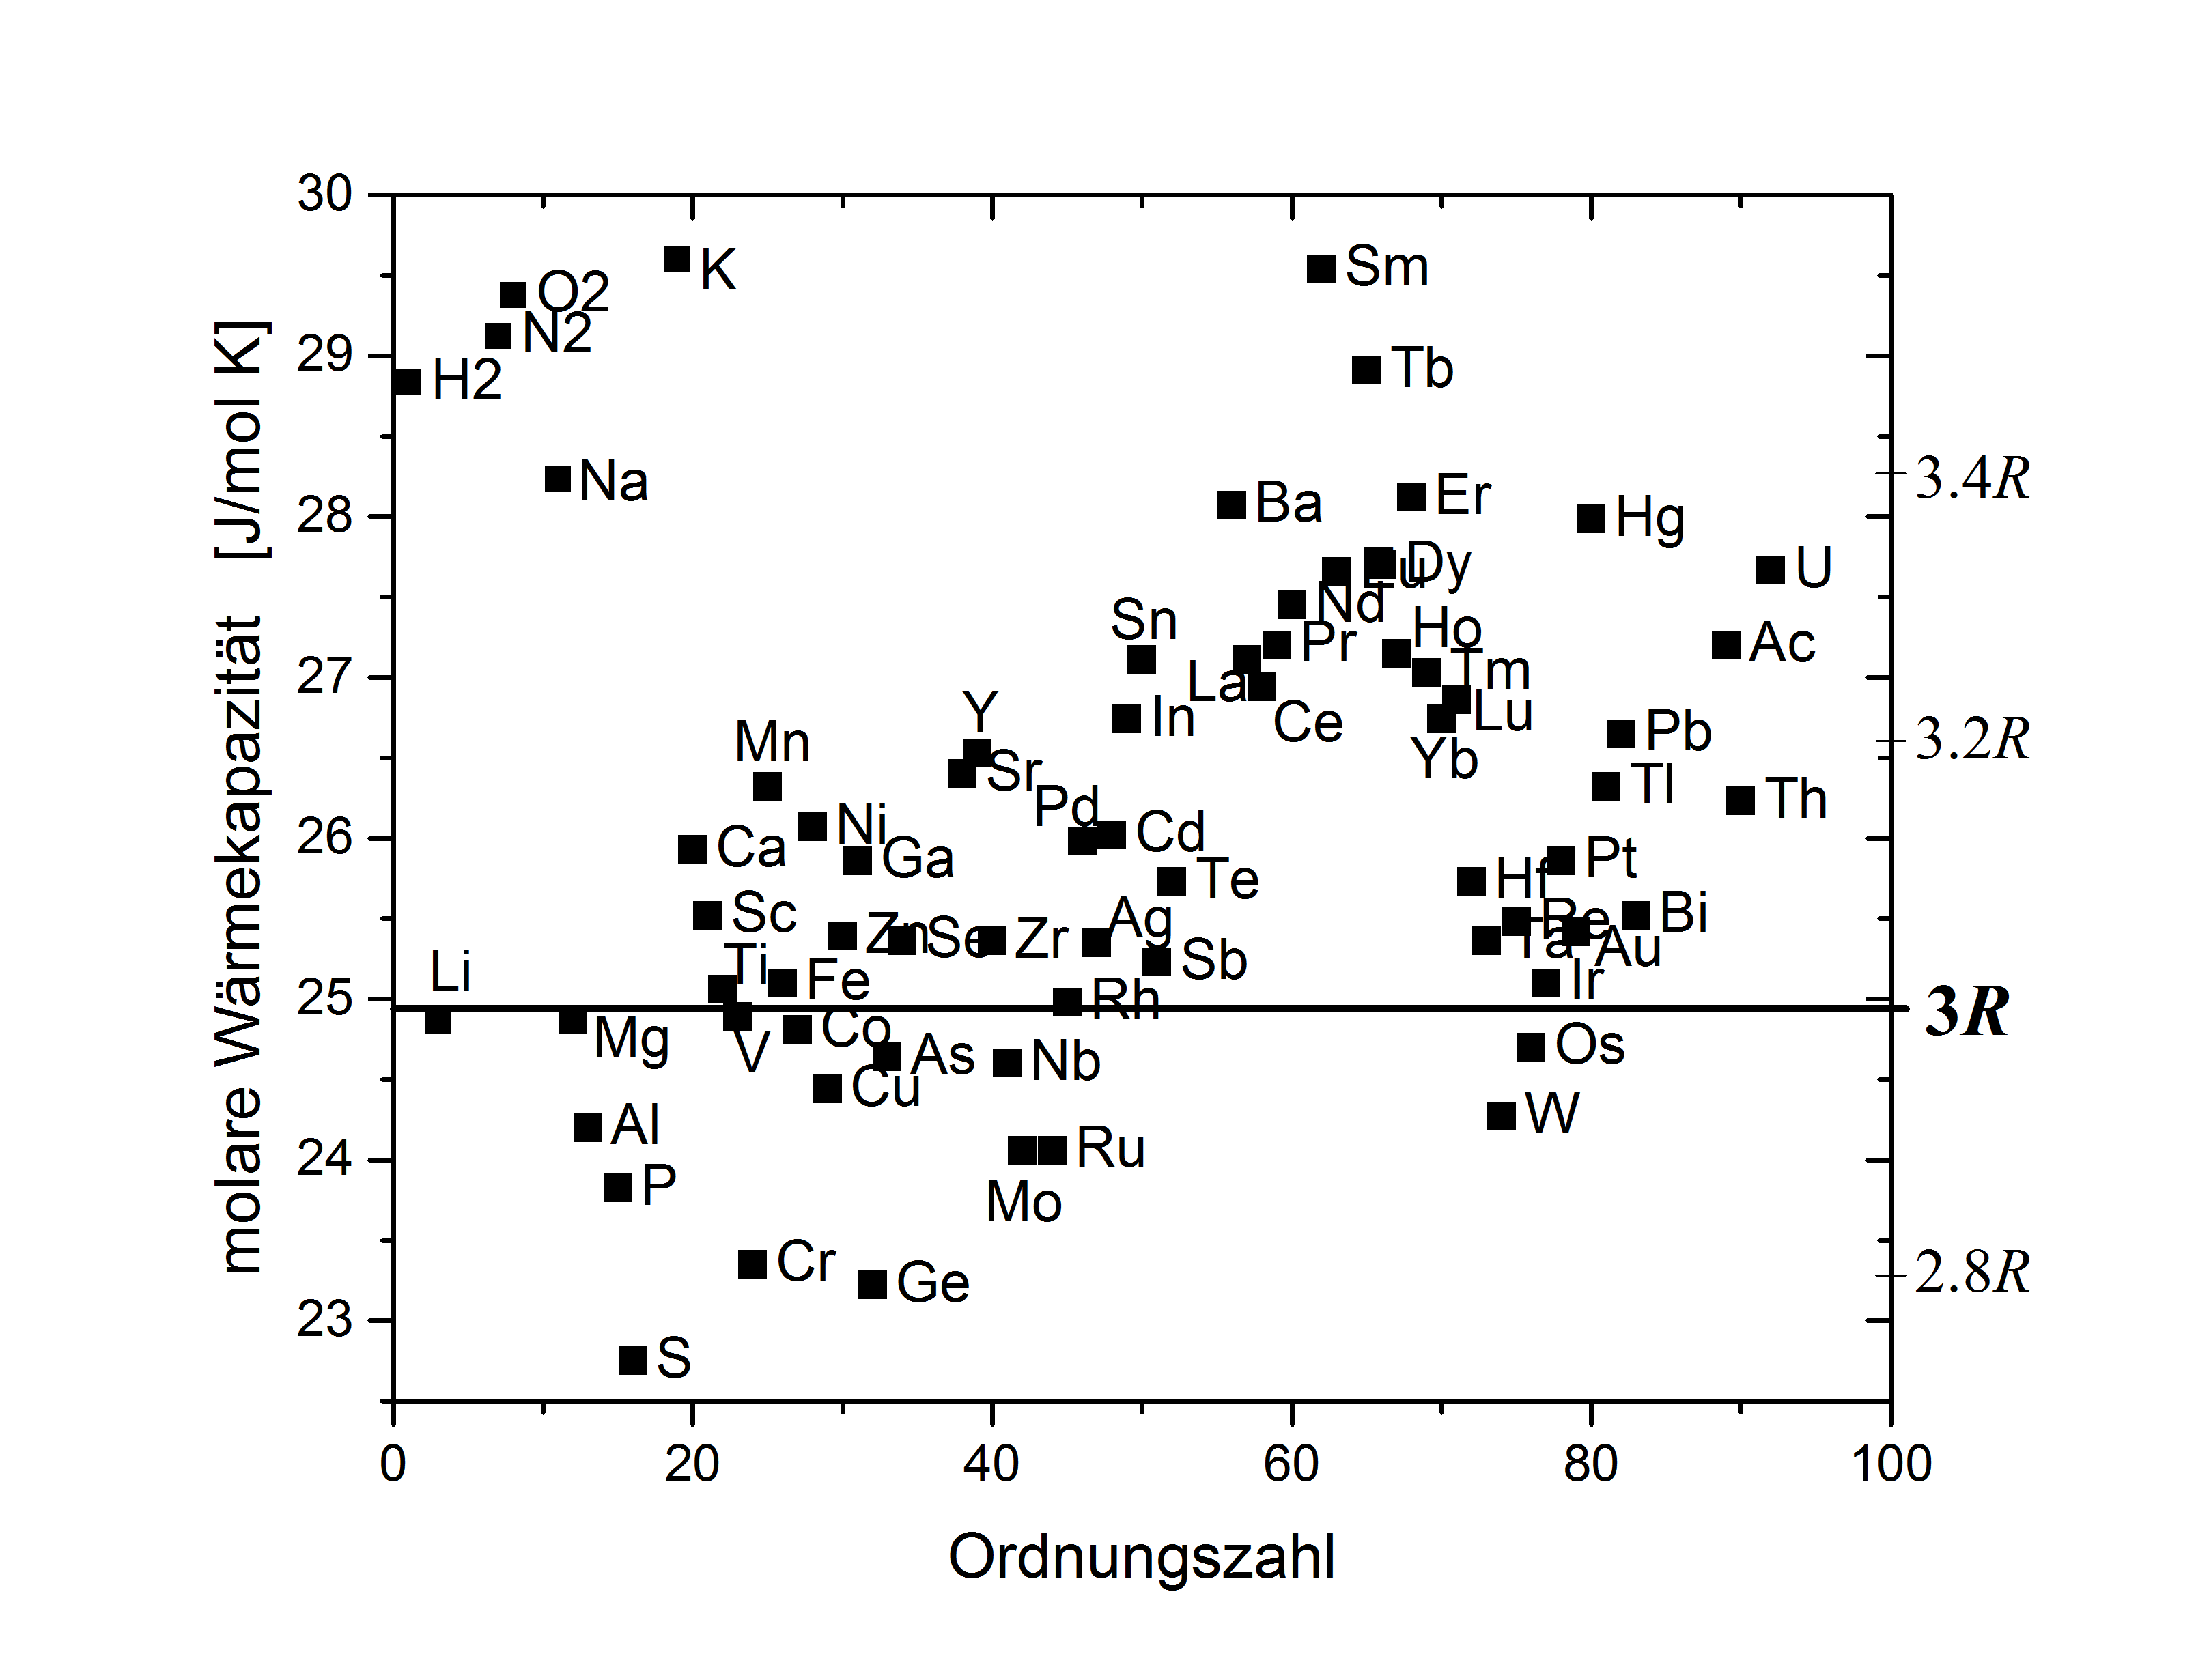
\includegraphics[width=\textwidth]{DP.png}
\caption{Molare Wärmekapazität aufgetragen gegen die Ordnungszahl. https://de.wikipedia.org/wiki/Dulong-Petit-Gesetz}
\end{figure}
\end{document}